\chapter{Introduction} \label{ch:chapter1}

This is a very short guide to an unofficial thesis/dissertation template for the University of Tennessee. It is based on the 2010 thesis specifications but can be easily altered as the guidelines are changed. This template requires a basic knowledge of \LaTeX\ and should cover the basic requirements in terms of required packages and functionality. This is a very short guide to an unofficial thesis/dissertation template for the University of Tennessee. It is based on the 2010 thesis specifications but can be easily altered as the guidelines are changed. This template requires a basic knowledge of \LaTeX\ and should cover the basic requirements in terms of required packages and functionality.

\begin{figure}[b!]
  \centering
  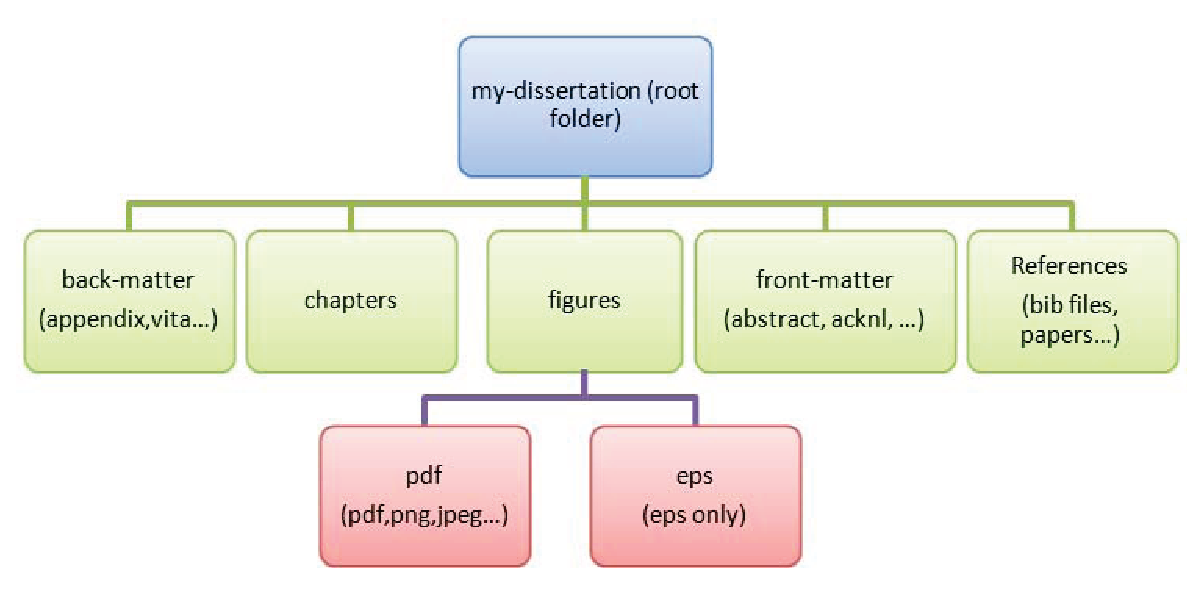
\includegraphics[width=6.5in]{fig01-folder-structure}\\
  \caption{UT thesis template folder structure.}\label{fig:intro-folder-structure}
\end{figure}
The general structure of this template is based on the tree shown in Figure \ref{fig:intro-folder-structure}. The titles of the folders are self descriptive and should guide you to proper file placement. Note that this is only a suggested model that could be modified to fit your own organizational structure.

\begin{verbatim}
%%%%%%%%%%%%%%%%%%%%%%%%%%%%%%%%%%%%%%%%%%%%%%%%%%%%%%%%%%%%%%%%%%%%%%%%%%%
Thesis, color, one side
\documentclass[thesis,monochrome,letterpaper,12pt]{utthesis}
Thesis, monochrome, one side
\documentclass[thesis,monochrome,letterpaper,12pt]{utthesis}
Thesis, color, twoside side (good for binding)
\documentclass[thesis,twoside,letterpaper,12pt]{utthesis}
Thesis, monochrome, twoside side (good for binding)
\documentclass[thesis,monochrome,twoside,letterpaper,12pt]{utthesis}
Dissertation, color, one side
\documentclass[dissertation,letterpaper,12pt]{utthesis}
Dissertation, monochrome, two side
\documentclass[dissertation,twoside,letterpaper,12pt]{utthesis} . . .
%%%%%%%%%%%%%%%%%%%%%%%%%%%%%%%%%%%%%%%%%%%%%%%%%%%%%%%%%%%%%%%%%%%%%%%%%%%
\end{verbatim}

\section{Theorem environments}
This template contains predefined theorem, lemma, and corollary environments. For example
\begin{theorem}[First theorem]\label{thm:theorem-a}
    This is an example theorem.
\end{theorem}
\begin{proof}[Proof for theorem] \ref{thm:theorem-a}
    This is the proof for this theorem.
\end{proof}
\begin{lemma}[First lemma]
    This is the first lemma.
\end{lemma}
\begin{corollary}
    This is the first corollary.
\end{corollary}

\subsection{Single figures}
For more information, check: \href{http://en.wikibooks.org/wiki/LaTeX/Floats,_Figures_and_Captions}{http://en.wikibooks.org/wiki/LaTeX/Floats,\_Figures\_and\_Captions}

\subsubsection{Testing}
In this part we tested some stuff.

\subsection{Multipart figures}
For multipart figures, you need to use the package "subfig". here's an example
\begin{figure}[h!]
        \centering
        \subfloat[Circle]{\label{fig:figure-a}
\includegraphics[width=1.1in]{fig02a-circle}}
        \subfloat[Rectangle]{\label{fig:figure-b}
\includegraphics[width=1.1in]{fig02b-rectangle}}
        \subfloat[Cube]{\label{fig:figure-c}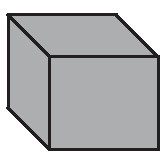
\includegraphics[width=1.1in]{fig02c-cube}}
        \caption{Geometric shapes.}
        \label{fig:multipart-figure}
\end{figure}
To add some space between the figures above, one can use the usual spacing commands such as ``qquad''
\begin{figure}[h!]
        \centering
        \subfloat[Circle]{\label{fig:figure-a}
\includegraphics[width=1.1in]{fig02a-circle}} \qquad
        \subfloat[Rectangle]{\label{fig:figure-b}
\includegraphics[width=1.1in]{fig02b-rectangle}}\qquad
        \subfloat[Cube]{\label{fig:figure-c}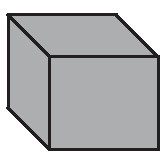
\includegraphics[width=1.1in]{fig02c-cube}}\qquad
        \caption{Geometric shapes.}
        \label{fig:multipart-figure}
\end{figure} 
